\chapter*{Methodology}
\addcontentsline{toc}{chapter}{Methodology}

In this section, the scenario setting of the project will be defined, and the theoretical methodology of the traditional SSL algorithm, DL-based SSL algorithm, and mobile platform will be described. The definition of the scenario setting is crucial for the purpose of research since different settings require different solutions. \\


The microphone array setting is tentatively described by the following:
\begin{enumerate}
    \item A hexagonal-shaped microphone array consists of six chip microphones, placed on a hexagonal 3D-printed foundation.
    \item The microphone center is defined as located at the origin of the microphone array coordinate system.
    \item The distance between the array center and each microphone is \(0.06m\).
    \item The geometry of the microphone array is shown below:
    \begin{figure}[H]
        \centering
        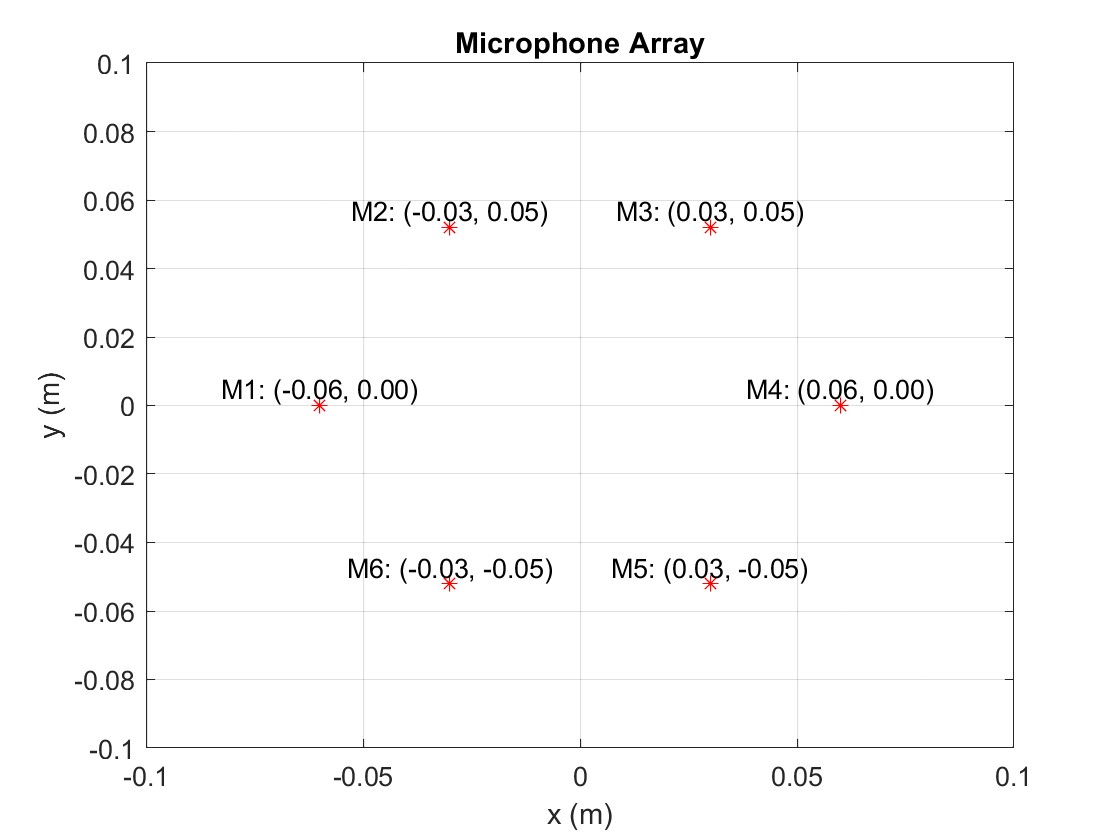
\includegraphics[width=0.8\linewidth]{figures/Geometry_microphone_array.jpg}
        \caption{The Geometry of the Hexagonal Microphone Array}
    \end{figure}
    \item The six microphones in the array are connected to a pre-processing PCB board which serves to combine the six channels signals into a USB serial port and to provide a buffer for the data. The apparatus of the microphone array is demonstrated below: 
    \begin{figure}[H]
        \begin{minipage}{0.45\textwidth}
                \centering
                \rotatebox[origin=c]{90}{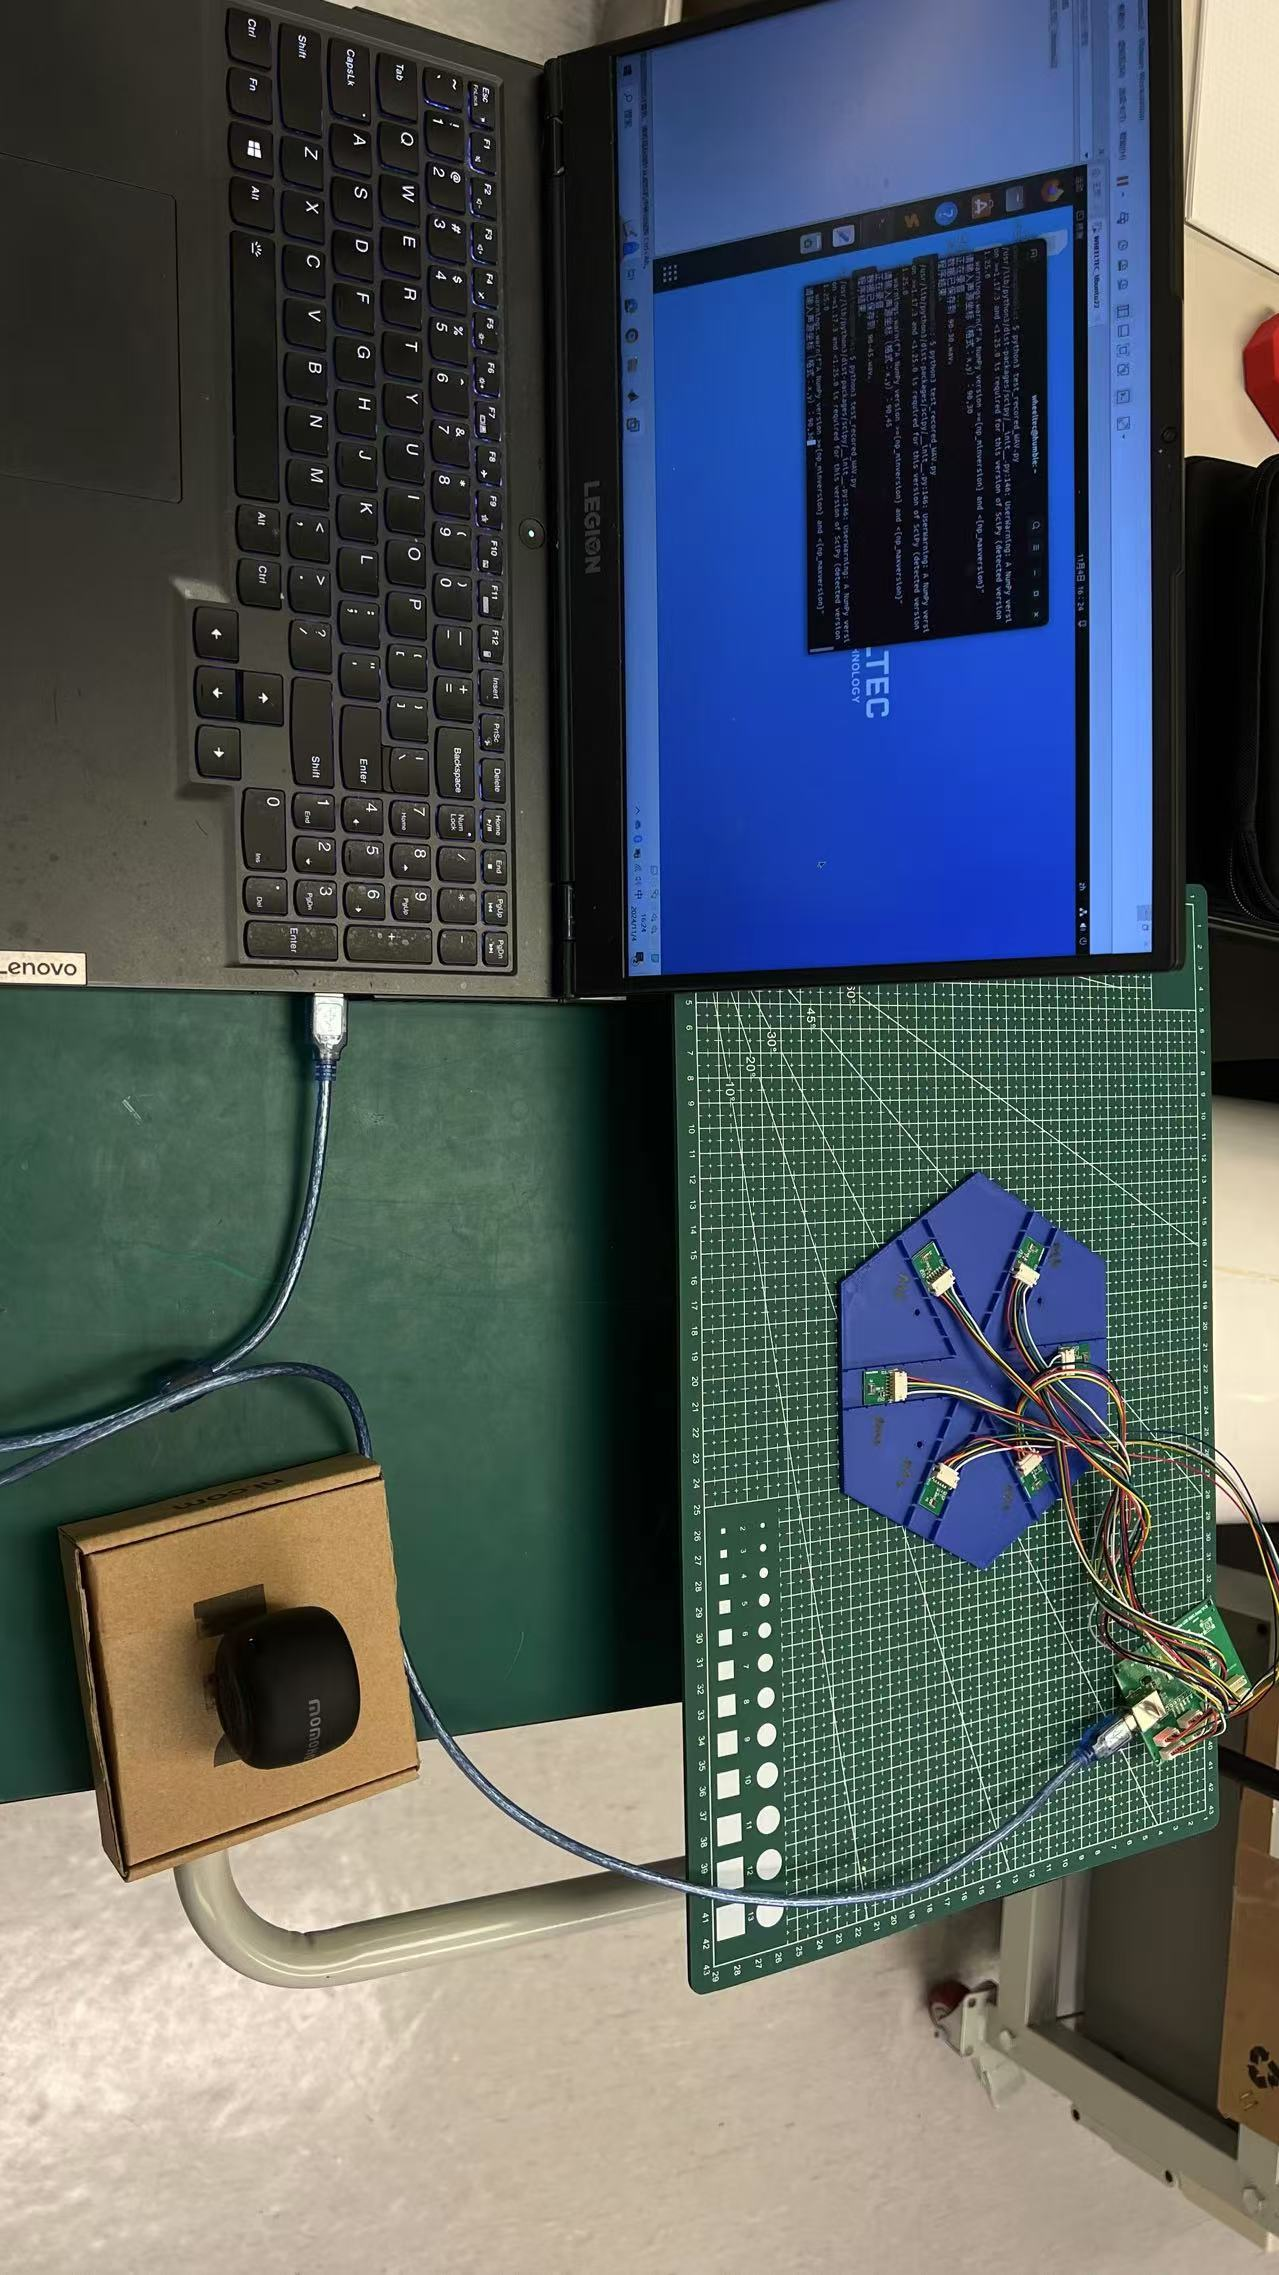
\includegraphics[width=0.5\linewidth]{figures/Microphone_array_photo.jpg}}
        \end{minipage}
        \begin{minipage}{0.45\textwidth}
                \centering
                \rotatebox[origin=c]{90}{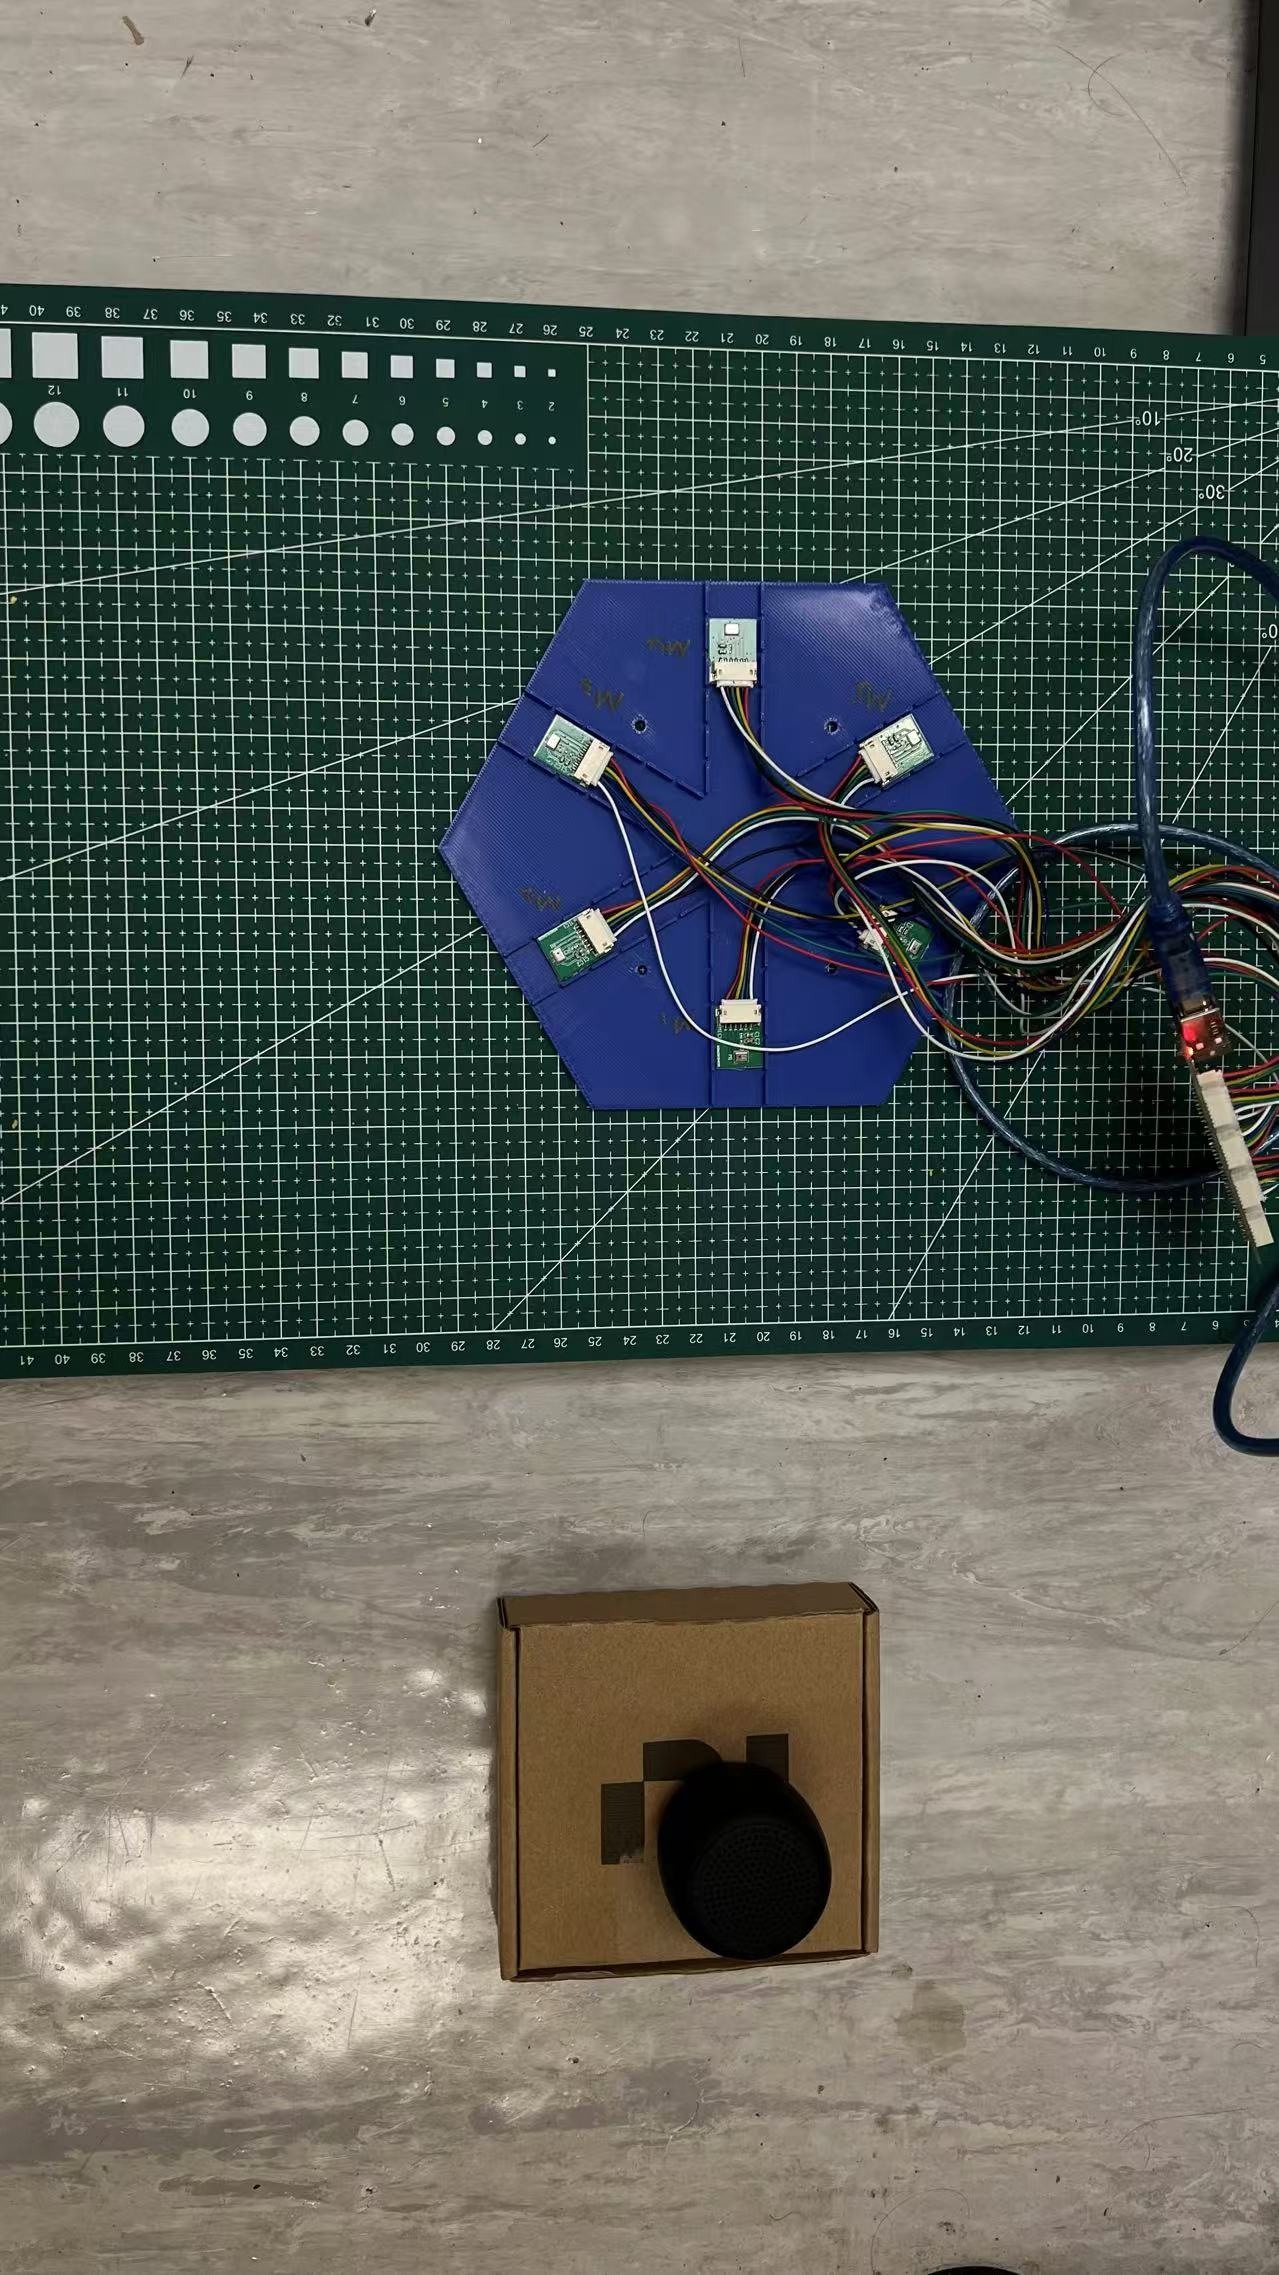
\includegraphics[width=0.5\linewidth]{figures/Microphone_array_photo_2.jpg}}
        \end{minipage}
        \caption{Hexagonal Microphone Array Apparatus}
    \end{figure}
\end{enumerate}

The setting of the SSL scenario is tentatively described by the following:
\begin{enumerate}
    \item The sound source is located \(0.3m\) to \(2m\) from the center of the microphone array. It is a blue-tooth speaker playing a human-speaking voice segment from the Librispeech dataset \cite{panayotov_resource_2015}.
    \item The sound source is located in the front of the microphone array, with its range of angle defined as \(\theta \in [0, \pi]\) in radius or \(\theta_d \in [0, 180]\) in degree. The unit circle defines the angle's orientation, which is counter-clockwise starting from the positive direction of the x-axis.
        
    \begin{figure}[H]
        \centering
        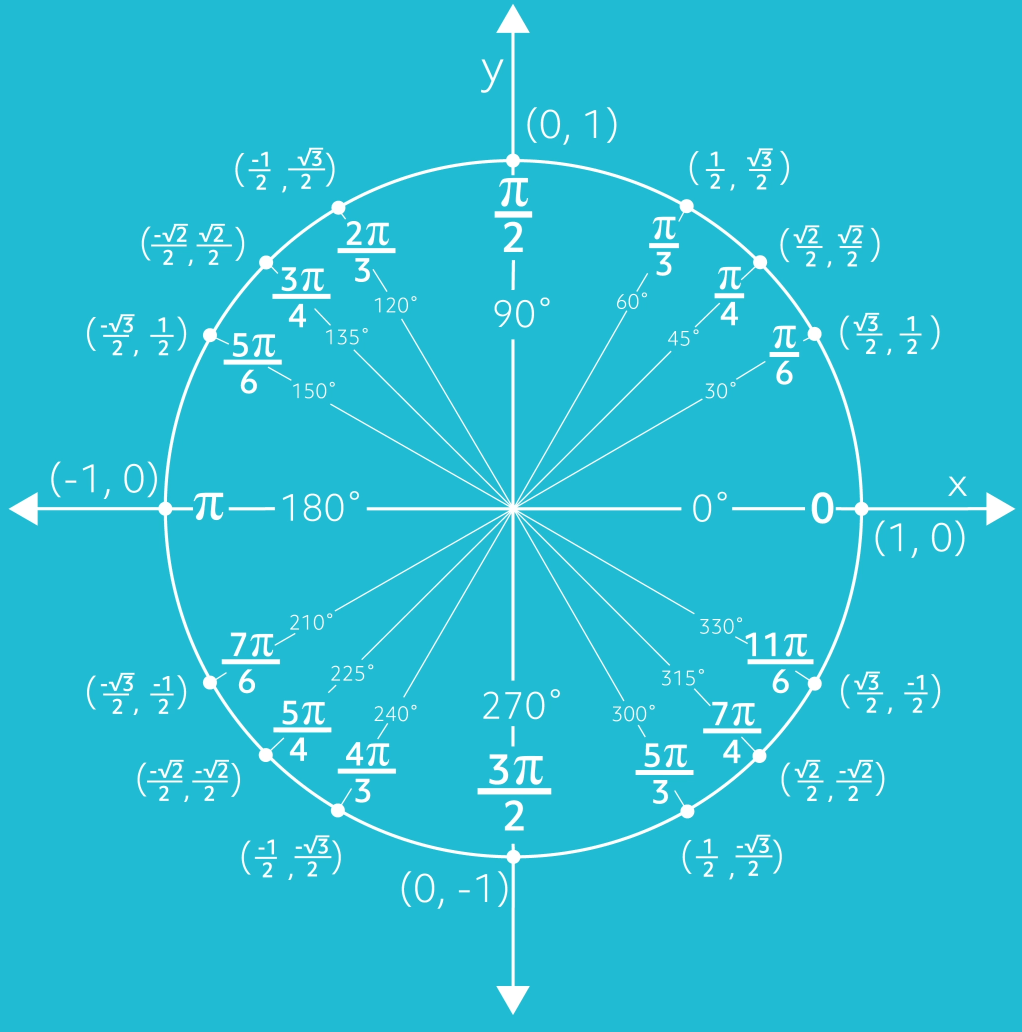
\includegraphics[width=0.3\linewidth]{figures/Unit_circle.png}
        \caption{Unit Circle}
    \end{figure}
    \item The distance between the center of the microphone array and the sound source is relatively large compared to the distances between microphones in the microphone array, indicating that the situation of the microphone array surrounding the sound source will not be considered.
    \item The surrounding environment is defined to be an indoor environment, indicating that complicated outdoor noises will not be involved. The non-reverberant situation will be first tested by utilizing the anechoic chamber. Future studies may include the reverberant situation if sufficient time exists.
    \item The input of the algorithm is defined as a ".wav" audio file, which will be further converted into two data:
    \begin{itemize}
        \item The sample rate of the audio file is expressed as \(f_s\) in \(Hz\), denoting the number of samples per second.
        \item The original multi-channel sound signal represented as a matrix:
        \[
            \mathbf{S} = 
            \begin{bmatrix}
                s_1(t)\\
                s_2(t)\\
                \vdots\\
                s_6(t)\\
            \end{bmatrix}
        \]
        In reality, it is represented in discrete form:
        \[
            \mathbf{S} = 
            \begin{bmatrix}
                s_{1,1} & s_{1,2} & \cdots & s_{1,t*f_s} \\
                s_{2,1} & s_{2,2} & \cdots & s_{2,t*f_s} \\
                \vdots & \vdots & \ddots & \vdots \\
                s_{6,1} & s_{6,2} & \cdots & s_{6,t*f_s} \\
            \end{bmatrix}
        \]
        where \(t\) stands for the total time of this audio file. The amplitude is represented by \(s_{c,n} \in [-32767, 32768]\), using the PCM16 audio file coding format.
        
    \end{itemize}
    \item The output of the algorithm should be the degree of arrival (DoA) on the plane of the microphone array, which is defined as the Azmith angle \(\theta\). The sound source is assumed to be located on the same plane of the array. The elevation angle will not be considered in this project.

\end{enumerate}

Notice that this is a tentative setting. Further adjustments may be included during future experiments if the developed algorithm demonstrates high robustness, accuracy, and performance.


\section*{Traditional SSL Methods (XIAO Pengbo)}
\addcontentsline{toc}{section}{Traditional SSL Methods (XIAO Pengbo)}


TDOA (Time Difference of Arrival) method, as one of the classic SSL (Sound Source Localization) method, performs excellently in environments with low noise and low reverberation. Its principle involves triangulating the position based on the time differences in the arrival of signals.

Assuming a system composed of two microphones located at coordinates \((x_1, y_1)\) and \((x_2, y_2)\), with the speed of sound in the current environment being \(c\). When a sound is emitted from the source and received by the two microphones, the TDOA value obtained is \(t_{12}\). Multiplying the TDOA value by \(c\) gives the distance difference between the sound source and the two microphones. Based on this, we can solve for the coordinates of the sound source:
\[
\sqrt{(x-x_{1})^{2}+(y-y_{1})^{2}}-\sqrt{(x-x_{2})^{2}+(y-y_{2})^{2}}=c*t_{1-2}
\]
Solving this equation, the result is a hyperbola representing all possible locations of the sound source under TDOA. By adding a third point, the intersection of two hyperbolas allows us to accurately determine the position of the sound source.\\
\begin{figure}[H]
    \centering
    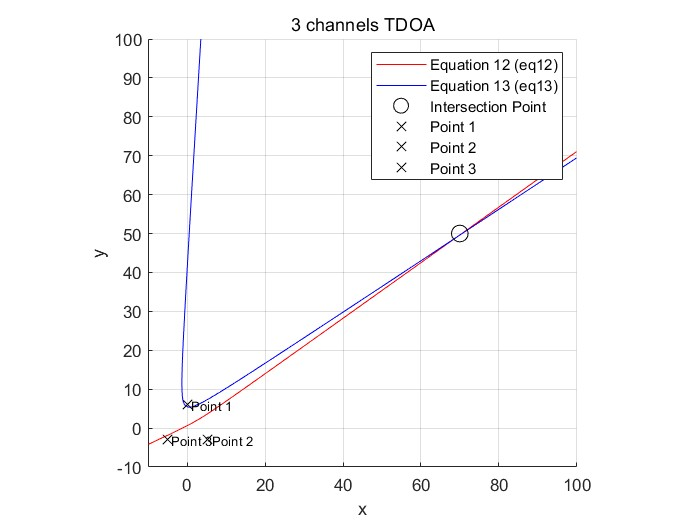
\includegraphics[width=0.7\linewidth]{figures/3_Channels.jpg}
    \caption{3-Channel TDOA Localization Schematic Diagram}
\end{figure}
Generally, there are two ways to obtain TDOA values: 

The first method involves subtracting the time of arrival (TOA) at each receiver. The limitation of this approach is that acquiring TOA requires strict synchronization between the signal source and the receivers. Therefore, this method is not suitable for locating randomly occurring signal sources in an environment.

The second method involves performing correlation calculations on the signals received by two receivers to obtain the TDOA value. This method does not require time synchronization between the sound source and the receivers, making it applicable in a wider range of scenarios and suitable for processing sporadic sound information in the environment. Therefore, this project employs the second method to solve for the TDOA value. 

In our project, the specific methods and principles are as follows:
\begin{enumerate}
    \item Collecting the sound pressure signals from each receivers while ensure all the receivers are time-synchronized. The signals are represented as the following matrix:
    \[
        \mathbf{S} = 
        \begin{bmatrix}
            s_1(t)\\
            s_2(t)\\
            \vdots\\
            s_6(t)\\
        \end{bmatrix}
    \]
    \(s_1\) to \(s_6\) is the signals of 6 channels (according to \textit{ The Geometry of the Hexagonal Microphone Array}, corresponding to M1 through M6).
    \item The project team divides the microphone array into 2 groups: M1 M3 M5 and M2 M4 M6. These two sets of signals, based on M1 and M2, are used for GCC (Generalized Cross-Correlation) calculation. The detail calculations are as following:
    
\end{enumerate}



\section*{Deep-Learning Based SSL Methods (ZENG Bailin)}
\addcontentsline{toc}{section}{Deep-Learning Based SSL Methods (ZENG Bailin)}


The SSL problem is defined as a classification problem instead of a regression problem. The algorithm input should be the original sound signal. The output of the DNN should be an array, with 180 elements representing the corresponding probability of DoA.\\
Notice that the development of the SSL deep learning model's structure is based on a current research project, \textit{Trusted Sound Source Localization} \cite{devin_sound_2024}.

\subsection*{Short-time Fourier Transform}
\addcontentsline{toc}{subsection}{Short-time Fourier Transform}
The feature extraction part Learning (DL) approach for sound source localization uses the Short-time Fourier Transform (STFT) projecting the time-domain multi-channel signal \(S\) to the time-frequency domain in the form of a spectrogram and processing the spectrogram using DNN. The STFT retains the audio signal variation with respect to time, as this variation may affect the result of the localization process. \\
The mathematical expression of the STFT is described as:
\[
    \textbf{STFT}_c(s_c(t), t,f) = \int_{-\infty}^{\infty} w(t-\tau) s_c(\tau) e^{-j2\pi f\tau}d\tau 
\]
where:
\begin{itemize}
    \item \(c\) is the index of microphone.
    \item \(w\) is a windowed function separating each time frame segment.
    \item \(t, f\) is the time and frequency in the final time-frequency domain. 
\end{itemize}
The discrete implementation of the STFT usually involves using the Fast Fourier Transform (FFT) to implement the transformation:
\[
    \textbf{STFT}_c(s_{c,n}, t, f) = \sum_{n = 1}^{N} s_{c,n} w(n-t) e^{-i2\pi k \frac{n}{N}}
\]
where:
\begin{itemize}
    \item \(s_{c,n}\) is the sample of the audio signal in channel \(c\) and sample index \(n\).
    \item \(N\) is the total number of samples, which should be \(N = t * f_s\).
\end{itemize}
Notice that in the application, this process is in discrete form, using summation instead of integration.
The resulting spectrogram is a time-frequency domain containing complex numbers, which contains the real part representing the amplitude, and the imaginary part representing the phase shift. Expressing in the form of a 3-dimensional tensor: \(\mathbf{X}_{ctf}\), where \(c\) is current microphone channels, \(f\) is frequency bin, and \(t\) is time frame.

However, during the implementation of the deep-learning process, the model should be able to understand the connection between the amplitude and phase shift for each time-frequency segmentation. Therefore, the imaginary parts are extracted from the original tensor \(\mathbf{X}_{ctf}\), transformed into real numbers, and concatenated along the channel dimension. The final shape of the resulting tensor, which is also the direct input of the DNN, should be:
\[
    \mathbf{X} \in \mathbb{R}^{2C\times F \times T}
\]
where \(C\) is the total number of microphone channels, \(F\) is the total number of frequency bins, and \(T\) is the total number of time frame.


\subsection*{Structure of the Deep-neural Network}
\addcontentsline{toc}{subsection}{Structure of the Deep-neural Network}
The structure of the DNN to process the result of STFT utilizes a combination of several structures, including Causal Convolution layers, 2-dimensional Max Pooling Layers,  Long short-term memory structure, and a fully connected layer. 
Defining the input of the DNN as:
\[
    \mathbf{X} \in \mathbb{R}^{B \times 2C\times F \times T}
\]
where \(B\) is the batch size per each propagation for the model's training purpose.\\
Tentatively, the architecture of the DNN's forward propagation is designed as the following:
\[
    \textbf{CRNN}(\mathbf{X}) = \textbf{FC}(\textbf{RNN}(\textbf{CNN}(\mathbf{X})))
\]
\textbf{CNN} is a convolution block including one layer of multi-head attention, further extracting important features from the multi-channel spectrogram \(\mathbf{X}\) and ignoring the unrelated feature. This block is formed by repeated 2-dimensional convolution block and 2-dimensional max-pooling processes in the time and frequency dimensions, expressed as:
\begin{align*}
    \textbf{CNN}(\mathbf{X}) = \textbf{MaxPool2d}(\textbf{CnnBlock}(\textbf{MaxPool2d}(\textbf{MultiHeadAttention}( \\
    \underbrace{\textbf{MaxPool2d}(\textbf{CnnBlock}(\ldots \textbf{CnnBlock}(\mathbf{X})\ldots}_{\text{3 times}}))))
\end{align*}
where the \textbf{MaxPool2d} is a 2-dimensional pooling layer, extracting the maximum number in a kernel. The \textbf{MultiHeadAttention} is a multi-head attention layer, correlating the information across the frequency dimension so that the model can comprehend information across different frequency bins.
The structure of the \textbf{CnnBlock} is given by:
\[
    \textbf{CnnBlock}(\mathbf{x}) = \textbf{Conv2d}(\textbf{BN}(\textbf{ReLU}(\textbf{Conv2d}(\mathbf{x})))
\]
where \textbf{Conv2d} is a standard 2-dimensional convolution layer, and \(\mathbf{x}\) is the output from the previous block and input of that block. \textbf{BN} is the batch normalization process, normalizing all the data along the batch dimension. \textbf{ReLU} is the rectified linear unit activation function.\\
The \textbf{RNN} is a standard long short-term memory layer (LSTM). Before entering the \textbf{RNN} layer, the tensor will be reshaped into a 3-dimensional tensor, and the frequency and channel dimensions will be combined:
\[
    \textbf{CNN(X)} = \mathbf{X}_{cnn,out} \in \mathbb{R}^{B \times 2C\times F' \times T'} \rightarrow \mathbf{X}_{rnn,in} \in \mathbb{R}^{B \times T' \times (F' \times 2C)}
\]
where the \(T'\) and \(F'\) are the total time frame and frequency bins after the \textbf{CNN} block. With the aid of the LSTM, the DNN should be able to comprehend the signal changes across the time frame. In case there are positional changes in the sound source, the model can correlate the sound source's position in the current time frame to the previous time frame. Meanwhile, through this LSTM process, the output dimension will be settled to 180:
\[
    \textbf{RNN}(\mathbf{X}_{rnn,in}) = \mathbf{X}_{rnn,out} \in \mathbb{R}^{B \times T' \times 180}
\]
The last layer of the model, the \textbf{RC}, is a fully connected layer, with its structure given by:
\[
    \mathbf{X}_{output} \in \mathbb{R}^{B \times T' \times 180} = \textbf{RC}(\mathbf{X}_{rnn,out}) = \textbf{Linear}(\textbf{Dropout}(\mathbf{X}_{rnn,out}))
\]
where the \textbf{Dropout} layer randomly discards data in neurons to prevent the over-fitting of the model, and the \textbf{Linear} layer is a linear mapping to the final output. The final output has three dimensions: the \(B\) is the batch size, \(T'\) is the convoluted time frames (the predicted time step), and \(180\) is the classes representing 180 degrees. The final resulting data is \(p \in \mathbb{R}\) representing the possibilities of sound sources existing in each class and each predicted time step.\\


\subsection*{Loss}
\addcontentsline{toc}{subsection}{Loss}
The loss function is crucial for the evaluation of the model's performance. The function takes in the predicted result and labels ground truth as inputs, and outputs the loss value representing the correctness of the prediction. It is used for the gradient descending process for the DNN training to adjust its parameters to approximate the ground truth, generating more trustworthy results.\\
In this DNN model, given the predicted output:
\[
    x_{b,t,c} = \mathbf{X}_{output} \in \mathbb{R}^{B \times T' \times 180} 
\]
and the labeled ground truth:
\[
    \mathbf{GT} \in \mathbb{R}^{B \times T'}
\]
where in each section of \(\mathbf{GT}\) there exists a DoA in radius representing the true DoA.\\
The cross-entropy function is used as the loss function. It involves several steps:
\begin{enumerate}
    \item Transform the ground truth from radius to degree:
    \[
        \text{GroundTruth}_{b,t} = \mathbf{GT}_{deg} = \mathbf{GT} \frac{180}{\pi}
    \]
    \item Generate truth label from the \(\mathbf{GT_{deg}}\):
    \[
        \text{one hot}(\mathbf{GT_{deg}}) = t_{b,t,c} = 
        \begin{cases}
        1 & \text{if } c = \text{GroundTruth}_{b,t}\\
        0 & \text{if } c \neq \text{GroundTruth}_{b,t}\\
        \end{cases}
        =\mathbf{T} \in \mathbb{R}^{B \times T' \times 180}
    \]
    where the result tensor \(\mathbf{T}\) has '1' for the correct class in each time frame, and '0' for each incorrect class.
    \item Apply the cross-entropy function to get the final loss for each time frame:
    \[
        loss_{b,t} = -\sum_{i = 1}^{180} t_{b,t,i} \log (x_{b,t,i}) = \mathbf{L} \in \mathbb{R}^{B \times T'}
    \]
\end{enumerate}

\subsection*{Prediction of DoA}
\addcontentsline{toc}{subsection}{Prediction of DoA}
Once the predicted tensor \(x_{b,t,c}\) is gained, the final prediction of DoA is given by:
\[
    \text{PredDoA}_{b,t} = \text{argmax}(x_{b,t,c}, \text{dim} = 2)
\]
The index of the class among the 180 classes will be returned for each batch and each time frame denoted as the DoA of prediction.\\

\subsection*{Computational Data Generation}
\addcontentsline{toc}{subsection}{Computational Data Generation}
The initial training process of the DNN utilizes computationally generated data, which can be gained at a lower cost than real-time recording. Meanwhile, different acoustic scenarios can be simulated by using the \textit{gpuRIR} \cite{diaz-guerra_gpurir_2021} and \textit{webrtcVAD} python libraries. During the data generation process, clean voice data from \textit{LibriSpeech} \cite{panayotov_resource_2015} will be segmented and integrated with noises from the dataset \textit{Noise92} \cite{andrew_assessment_1993}. The \textit{webrtcVAD} library is utilized to detect whether the segmentation contains noise, removing the empty segment from the dataset. The \textit{gpuRIR} \cite{diaz-guerra_gpurir_2021} is utilized to simulate the sound transmission process, generating the final signal received by each microphone channel. The \textit{gpuRIR} \cite{diaz-guerra_gpurir_2021} can also be used to simulate room reverberation and high reverberant cases will be considered in future testing if the model can process the non-reverberation case properly.\\
During the data generation process, the DoA will be selected randomly, and the clean voice segmentation and noise will be used to ensure the model adapts to various acoustic situations.\\
Three datasets will be generated: one for the training of the DNN, one for accuracy validation after each training epoch, and one for the final testing of the model's performance.

\subsection*{The Training Process}
\addcontentsline{toc}{subsection}{The Training Process}
All the parameters in the previously mentioned structures are to be changed during the model training process, which uses labeled ground truth and the backward propagation process to adjust these parameters to fit the training data. \\
The entire training process will be divided into epochs, and each epoch will be divided into steps. During one epoch, the DNN will process all the labeled data in the training dataset and a validation process will be conducted at the end of the one epoch, using the validation dataset to verify the result of this epoch. For each step, one batch, containing the number of data equal to the batch size, will be processed once through the DNN, including forward propagation and backward propagation, and the parameters will be adjusted once at the end.\\
After a given number of epochs, the training process is regarded as finished, and the testing dataset will be used to measure the prediction performance of the model.


\section*{Mobile Platform (WU Zhuoli)}
\addcontentsline{toc}{section}{Mobile Platform (WU Zhuoli)}

\input{chapters/methodology/mobile_platform}